\documentclass[conference]{IEEEtran}
\IEEEoverridecommandlockouts

\usepackage{amsmath,amssymb}
\usepackage{graphicx}
\usepackage{booktabs}
\usepackage{array}
\usepackage{hyperref}

\title{Learning Chaotic Continuous-Time Dynamics on the Lorenz System: Numerical Simulation, Short-Horizon Forecasting, and Attractor Reconstruction}

\author{
\IEEEauthorblockN{Scientific Machine Learning Course Project}
}

\begin{document}
\maketitle

\begin{abstract}
Chaotic continuous-time systems are a demanding benchmark for Scientific Machine Learning because strong local prediction does not guarantee correct long-term dynamics. We study this issue on the Lorenz system by comparing classical numerical simulation, a one-step multilayer perceptron (MLP), a residual discrete-time predictor, and a Neural ODE. The residual model achieves the best one-step mean-squared error, while the Neural ODE achieves the best rollout RMSE at horizons 50, 100, and 500. The experiments show that evaluating chaotic dynamics requires both local predictive accuracy and global dynamical fidelity through rollout behavior and attractor reconstruction.
\end{abstract}

\section{Introduction}
Scientific Machine Learning (SciML) is especially compelling when machine learning is used to approximate the behavior of a known physical or mathematical dynamical system. In this project, we use the Lorenz equations as a benchmark because they are low-dimensional, visually interpretable, and chaotic under the standard parameter choice. This makes them ideal for showing a central issue in learning dynamical systems: a model can perform well on one-step supervised prediction while still failing to preserve the correct long-term geometry.

Our goal is to compare three learning paradigms on the same reproducible pipeline:
\begin{enumerate}
\item a discrete-time MLP next-state predictor,
\item a residual discrete-time model that predicts state increments,
\item a Neural ODE that learns a continuous-time vector field.
\end{enumerate}

The main question is not only which model predicts best locally, but which model best reflects the underlying dynamics over rollout horizons and attractor-level diagnostics.

\section{Lorenz System and Dataset}
We study
\begin{equation}
\dot{x} = \sigma (y-x), \qquad
\dot{y} = x(\rho-z)-y, \qquad
\dot{z} = xy - \beta z
\end{equation}
with $(\sigma,\rho,\beta)=(10,28,8/3)$. The state is $s(t)=[x(t),y(t),z(t)]^\top$. Under this parameter setting, nearby trajectories diverge rapidly while remaining confined to the butterfly-shaped attractor.

\begin{figure}[t]
\centering
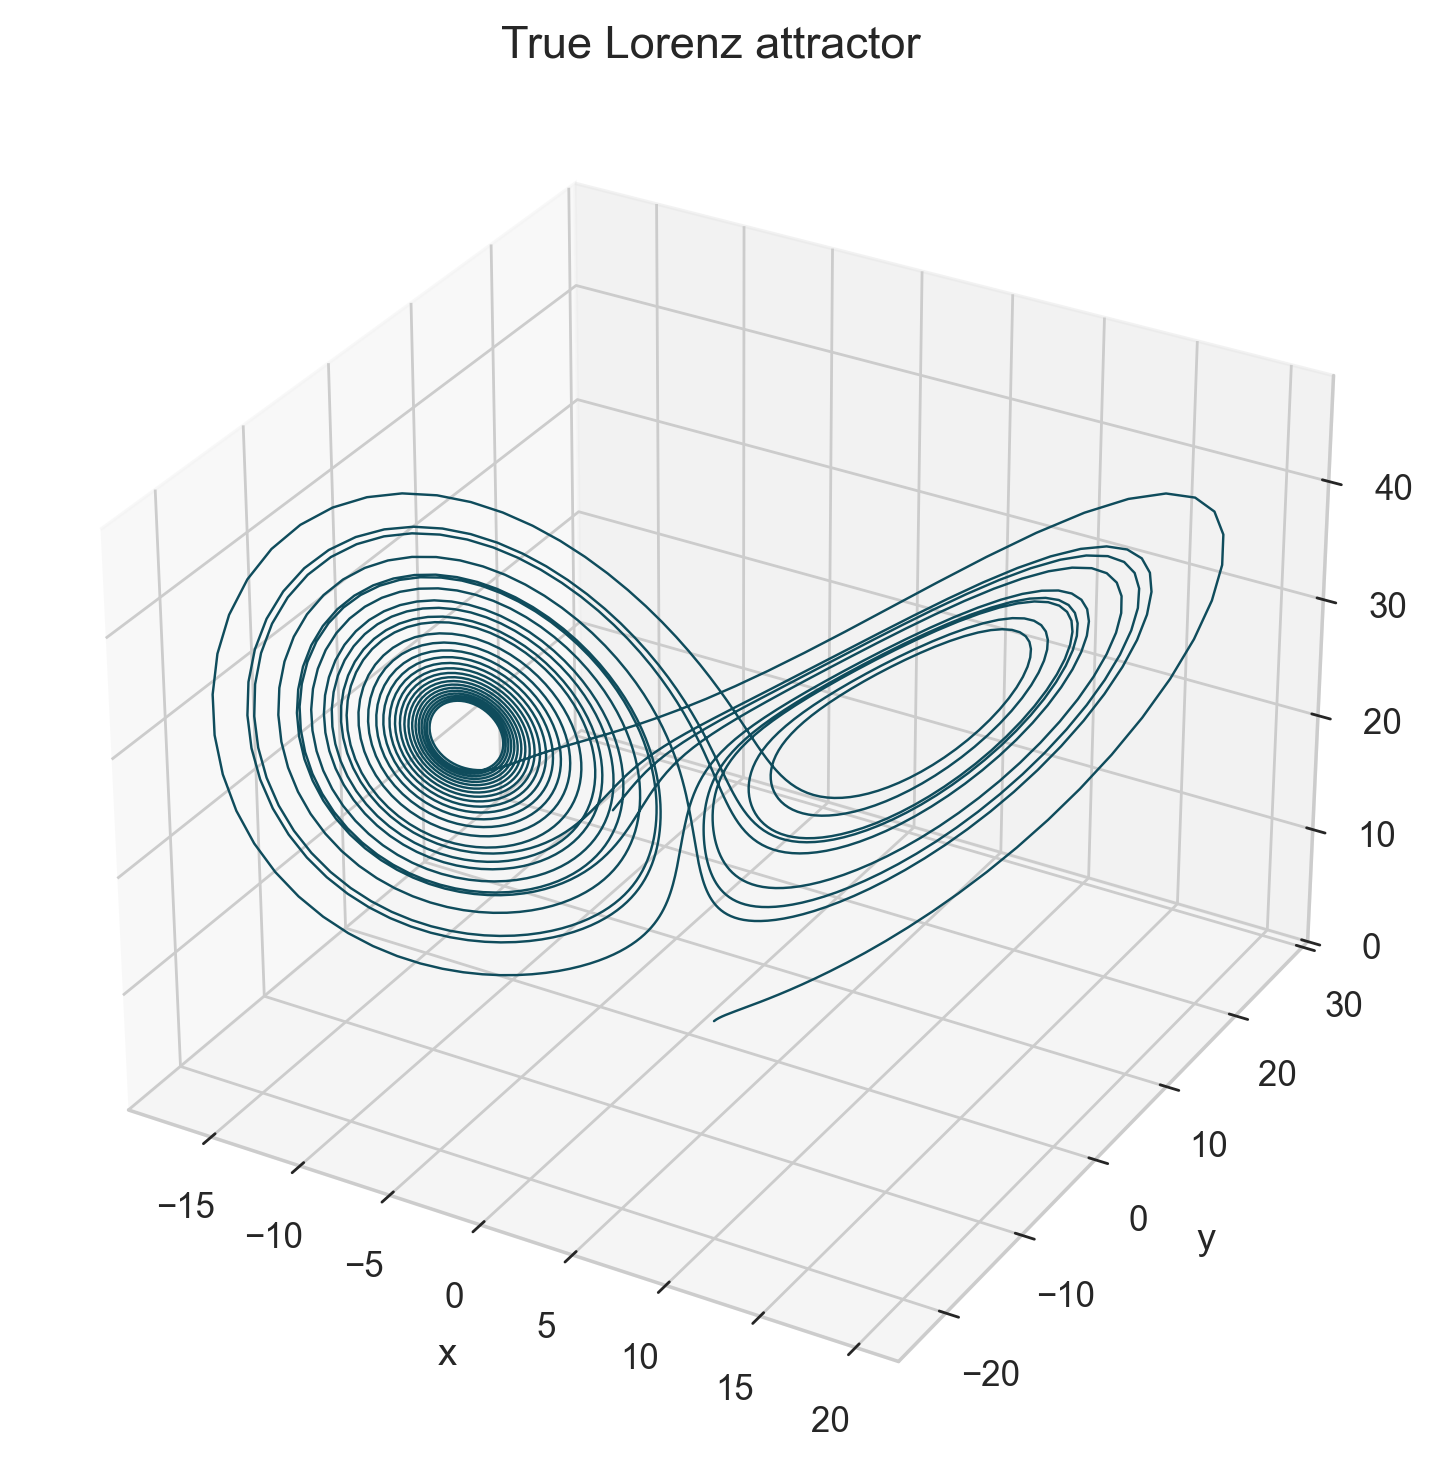
\includegraphics[width=\columnwidth]{results/report_assets/figure_true_attractor.png}
\caption{Reference Lorenz attractor under the standard chaotic parameter setting.}
\label{fig:lorenz_attractor}
\end{figure}

Reference trajectories were generated with a fixed-step RK4 solver. The default dataset contains 100 training trajectories, 20 validation trajectories, and 20 test trajectories, each simulated over $T=25$ with $\Delta t=0.01$. Splits were made by trajectory rather than by individual time points to avoid temporal leakage.

\section{Models}
\subsection{Discrete-Time Baselines}
The MLP baseline learns a map from $s_t$ to $s_{t+1}$. During rollout, its own predictions are recursively fed back as inputs. The residual model instead learns a state increment $\Delta s_t$ and predicts
\begin{equation}
s_{t+1} \approx s_t + \Delta s_t.
\end{equation}
This parameterization is often better aligned with discretized dynamics.

\subsection{Neural ODE}
The Neural ODE learns a continuous-time vector field
\begin{equation}
\dot{s} = f_\theta(s),
\end{equation}
where $f_\theta$ is represented by a neural network. Predicted trajectories are obtained by numerically integrating the learned vector field. This is the most explicitly SciML component of the project because the model structure mirrors the original scientific formulation.

\section{Evaluation Protocol}
Chaotic forecasting should not be judged by one metric alone. We therefore evaluate:
\begin{itemize}
\item one-step MSE and MAE,
\item rollout RMSE at horizons 50, 100, and 500,
\item attractor occupancy similarity through a coarse density distance,
\item qualitative phase portraits and attractor projections,
\item robustness under observation noise and time-step shifts.
\end{itemize}

This protocol distinguishes local predictive accuracy from global dynamical fidelity.

\section{Results}
Table~\ref{tab:main_results} summarizes the main quantitative outcomes. The residual predictor achieved the best one-step MSE, showing that increment prediction is a strong local parameterization for the Lorenz flow map. However, the Neural ODE achieved the lowest rollout RMSE at horizons 50, 100, and 500, which indicates better short- and medium-horizon behavior. This difference is exactly the SciML point of the project: the best one-step learner is not necessarily the best dynamical model.

\begin{table}[t]
\caption{Main test metrics on the Lorenz benchmark.}
\label{tab:main_results}
\centering
\footnotesize
\begin{tabular}{lcccc}
\toprule
Model & One-step MSE & RMSE$_{50}$ & RMSE$_{100}$ & RMSE$_{500}$ \\
\midrule
MLP & $3.72{\times}10^{-4}$ & 0.731 & 0.894 & 6.395 \\
Residual & \textbf{$5.71{\times}10^{-5}$} & 0.510 & 0.641 & 6.842 \\
Neural ODE & $2.18{\times}10^{-4}$ & \textbf{0.438} & \textbf{0.622} & \textbf{6.011} \\
\bottomrule
\end{tabular}
\end{table}

The direct MLP learned accurate local transitions but showed weaker recursive rollout performance than the structured alternatives. The residual model dramatically improved one-step accuracy and remained competitive on short rollouts. The Neural ODE, while not the strongest one-step predictor, most consistently matched continuous-time behavior under rollout evaluation.

Training cost also reflected the added structure. The MLP and residual models each used 33,923 trainable parameters, whereas the Neural ODE used 17,411 parameters but took longer to train because each forward pass involved numerical integration. In our experiments, approximate training times were 12.7 minutes for the MLP, 20.2 minutes for the residual model, and 24.7 minutes for the Neural ODE.

\begin{figure}[t]
\centering
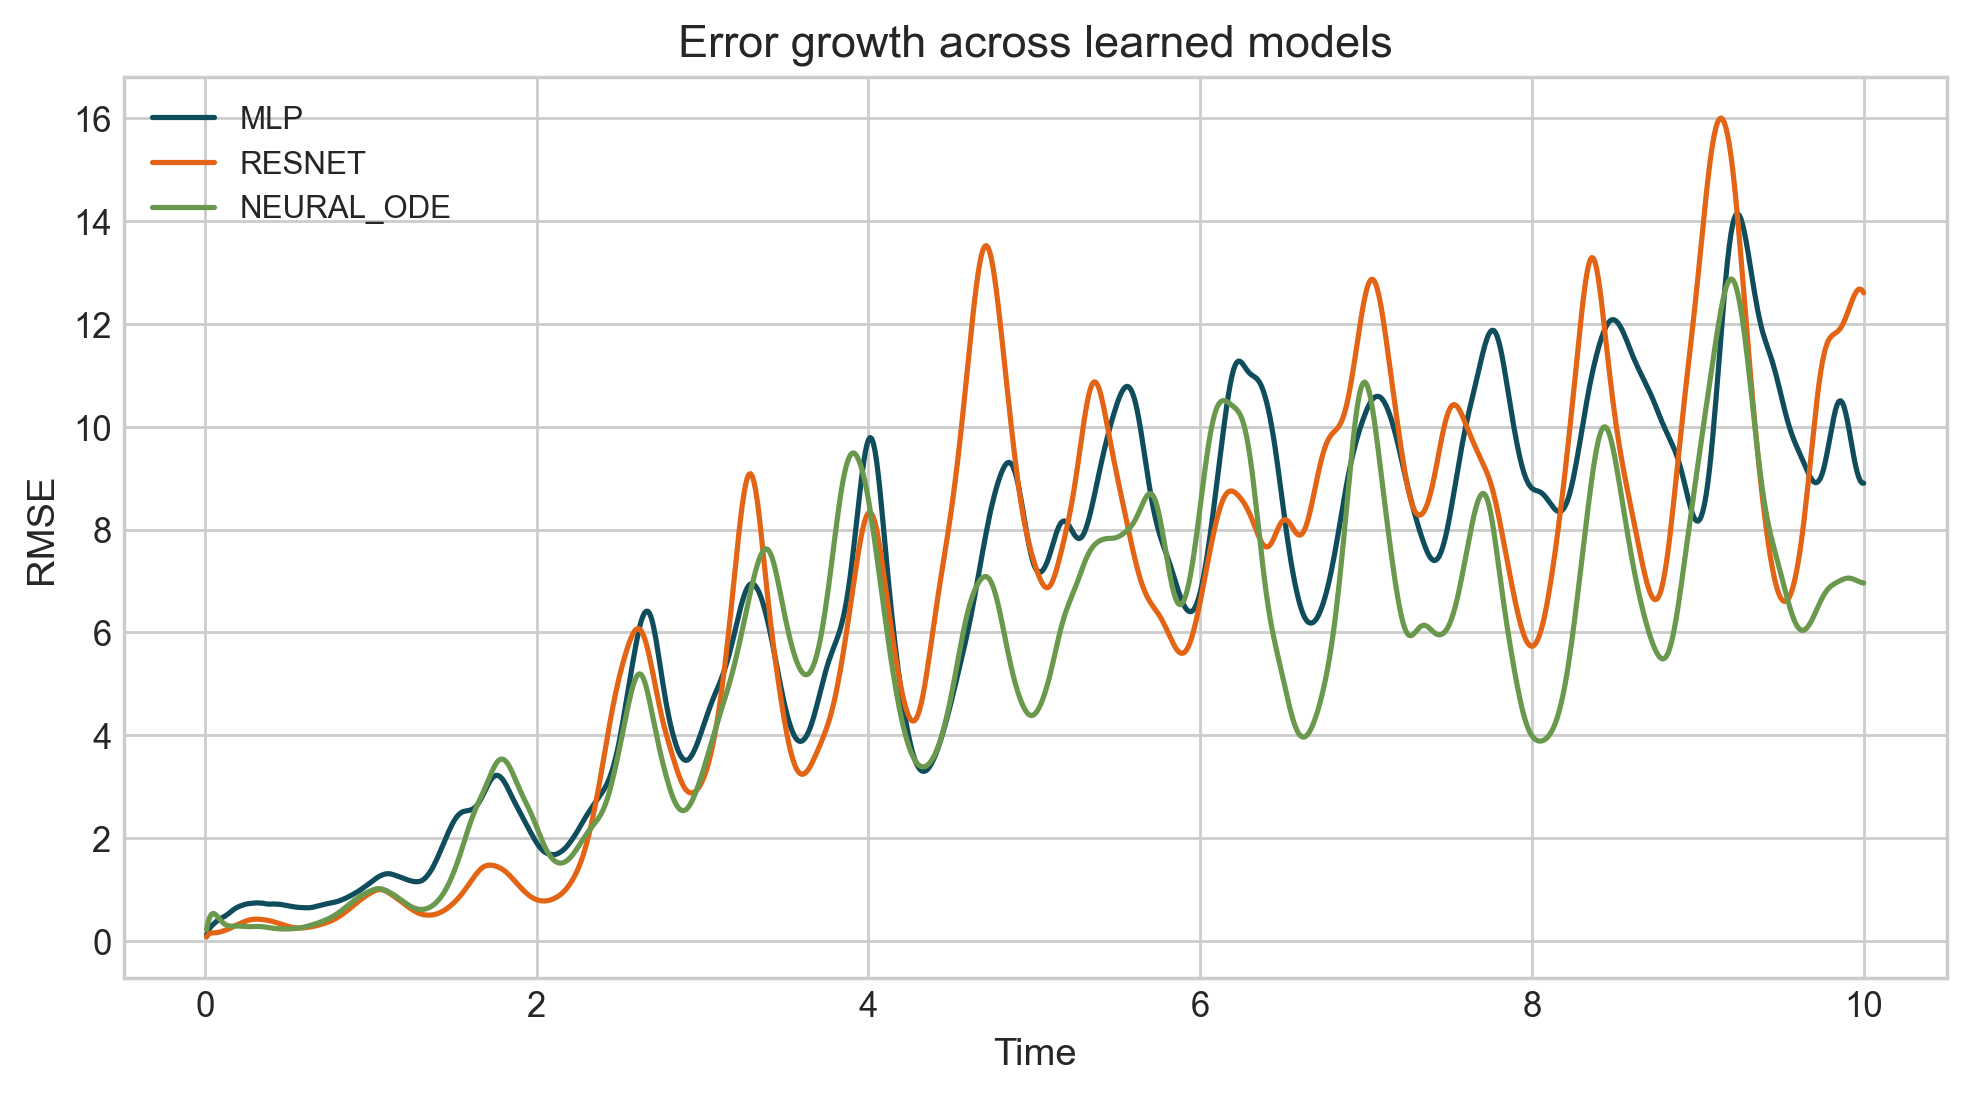
\includegraphics[width=\columnwidth]{results/report_assets/figure_error_growth_all_models.png}
\caption{Rollout error growth across the learned models. The Neural ODE remains best over the evaluated horizons even though it is not the best one-step predictor.}
\label{fig:error_growth}
\end{figure}

Qualitative figures supported the same interpretation. All models eventually deviated from exact test trajectories, which is expected under chaos. However, the residual model and Neural ODE recovered the butterfly geometry more faithfully than the plain MLP. This is why attractor reconstruction and phase portraits are more meaningful long-horizon diagnostics than pointwise tracking alone. Figure~\ref{fig:error_growth} makes the same point quantitatively: short-horizon differences are modest, but dynamical quality separates more clearly as the rollout length increases.

\section{SciML Interpretation}
This project is a SciML study, not just a standard forecasting benchmark, for three reasons. First, the target system is a scientific continuous-time ODE. Second, the learning pipeline is grounded in numerical simulation rather than arbitrary tabular data. Third, the evaluation is dynamical: the learned models are judged by rollout behavior, attractor structure, and robustness, not only by one-step loss.

The Neural ODE is the clearest example of this perspective. It learns a vector field directly and uses integration during both training and inference. Even though it does not produce the best one-step MSE, it provides the strongest rollout RMSE and naturally supports step-size-sensitive reasoning.

\begin{figure}[t]
\centering
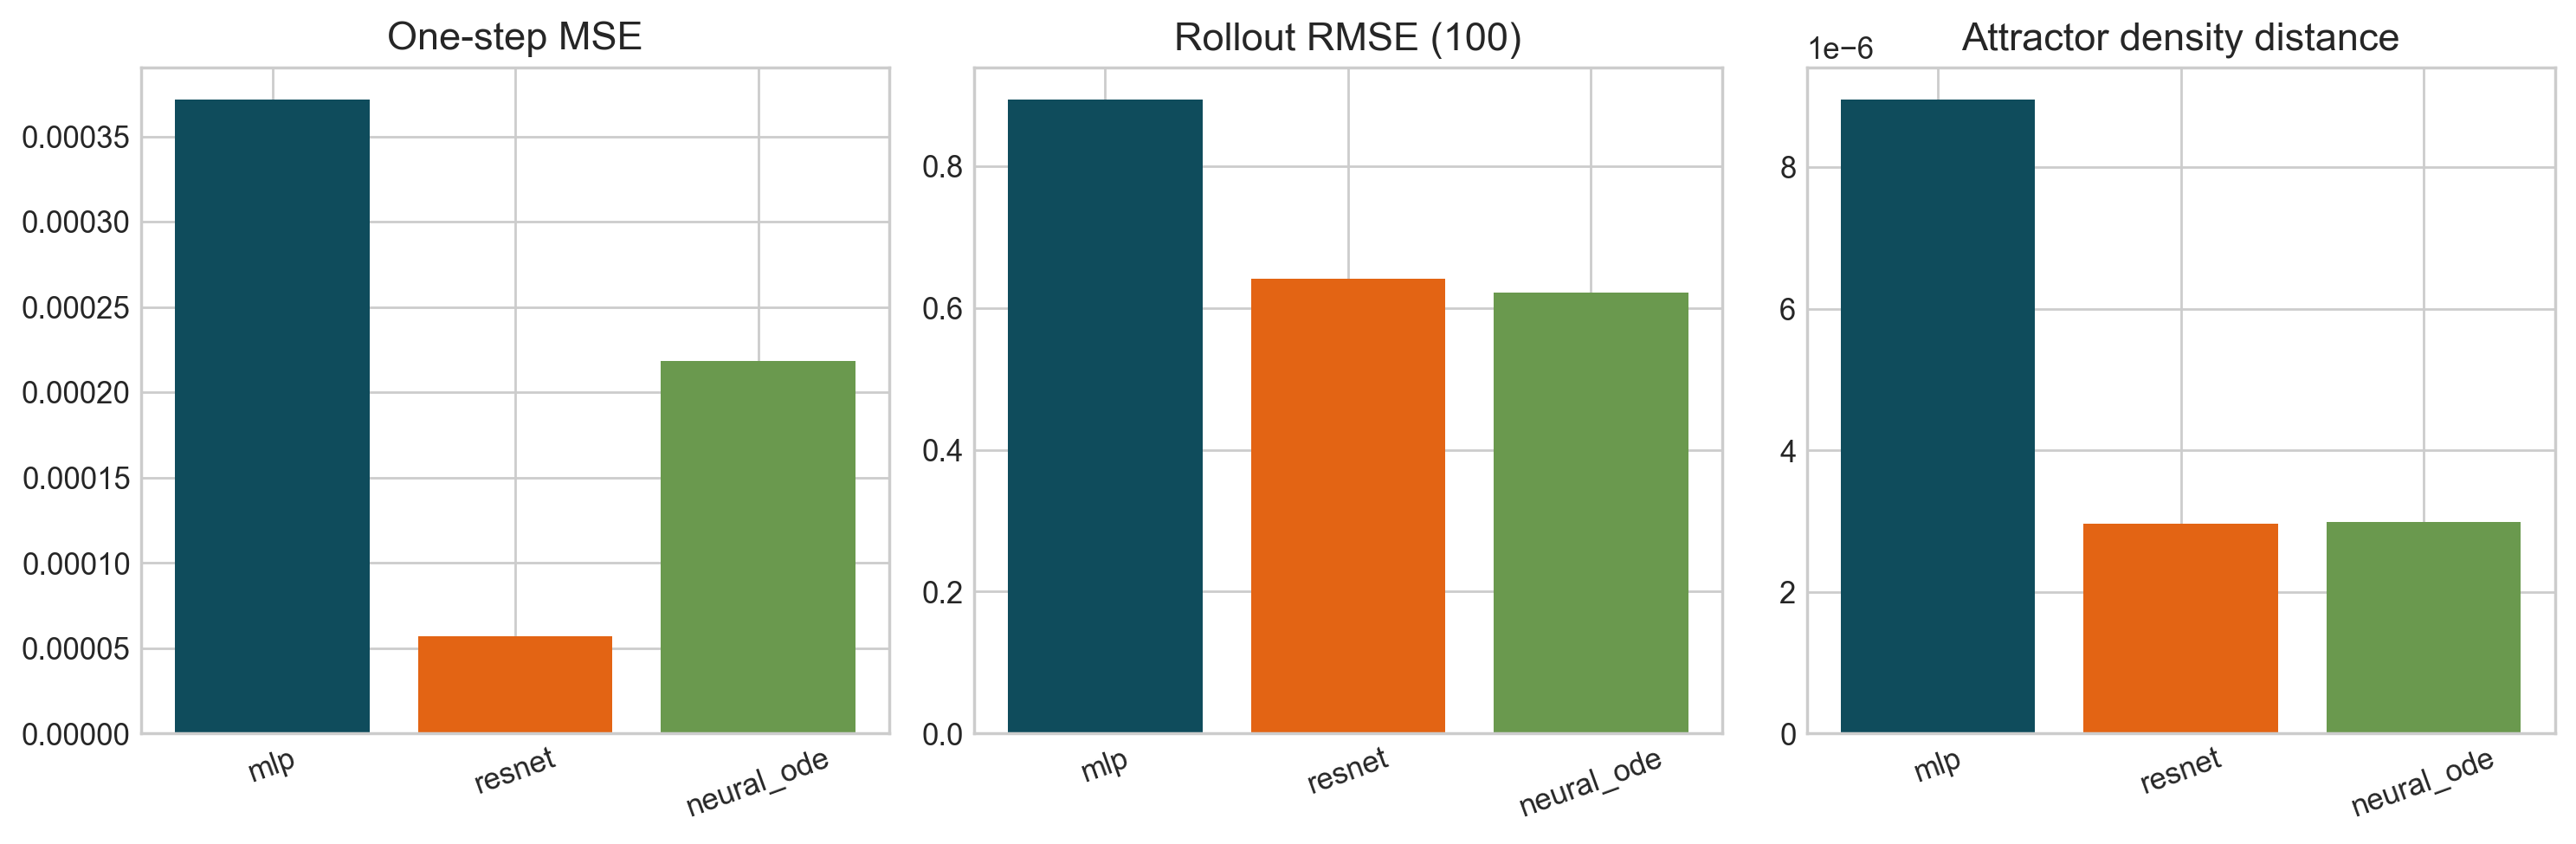
\includegraphics[width=\columnwidth]{results/report_assets/figure_final_summary.png}
\caption{Compact summary of one-step, rollout, and attractor-level comparisons across the three learned models.}
\label{fig:final_summary}
\end{figure}

\section{Conclusion}
The Lorenz benchmark clearly demonstrates that one-step prediction can be misleading for chaotic systems. The residual predictor was best for local forecasting, but the Neural ODE was best for rollout accuracy over the tested horizons and better aligned with the continuous-time nature of the problem. The main lesson is that learned chaotic dynamics should be evaluated with both predictive and dynamical criteria. As summarized in Fig.~\ref{fig:final_summary}, preserving the qualitative geometry of the system is as important as minimizing immediate prediction error.

\end{document}
